\documentclass{article}	
%\usepackage{times}
\usepackage{amsmath}
\usepackage{graphicx}
\usepackage{myapalike}

%\renewcommand{\rmdefault}{phv}
%\renewcommand{\ttdefault}{phv}

\hoffset-2cm
\addtolength{\textwidth}{3cm}
%\voffset-1cm
\addtolength{\textheight}{2cm}

\makeatletter
\newenvironment{myenum}{
% \renewcommand{\theenumi}{\roman{enumi}}
% \renewcommand{\labelenumi}{(\theenumi)}
\begin{list}{\labelenumi}{\setlength{\leftmargin}{1.3em}
  \setcounter{enumi}{0}
  \renewcommand{\item}{\addtocounter{enumi}{1}\unskip \vspace{-0.1cm}\@inmatherr\item
  \@ifnextchar [\@item{\@noitemargtrue \@item[\@itemlabel]} \unskip}}
  \itemsep0.1cm plus0.1cm minus0.05cm
  \listparindent0cm
  \setlength{\labelsep}{0.5em}
  \setlength{\labelwidth}{0.8em}}
{\end{list}}
\makeatother

\newenvironment{myitem}{\begin{list}{$\bullet$}{\setlength{\leftmargin}{1.1em}
\itemsep0.1cm plus0.1cm minus0.05cm
\listparindent0cm
\addtolength{\labelsep}{0.5\labelsep}
\setlength{\labelwidth}{0.8em}
\setlength{\leftmargin}{\labelwidth}
\addtolength{\leftmargin}{\labelsep}
}}{\end{list}}


\begin{document}

\begin{titlepage}
  \begin{center}
  {{\bf \Large 
    StdpC 2007 }\\[0.3cm]
    \large (Spike timing dependent plasticity Clamp)}, \\[1cm]
  {\large 
    in parts based on {\bf DYNCLAMP2} \cite{Pinto2001} 
  } \\[2cm]
  {\sc \Large Manual }
  \end{center}
\vspace*{5cm}

\noindent
{\large Thomas Nowotny} \\[0.5cm]
Centre for Computational Neuroscience and Robotics, \\
Department of Informatics, \\
University of Sussex, \\
Brighton BN1 9QJ, UK \\
E-mail: t.nowotny@sussex.ac.uk
September 2008, \\[1cm]
Original DYNCLAMP2 developers: \\[0.2cm]
Reynaldo Daniel Pinto, \\
Robert C. Elson, \\
Attila Sz\"ucs, \\
M. I. Rabinovich, \\
A. I. Selverston,  \\
H. D. I. Abarbanel \\[0.5cm]
Institute for Nonlinear Science, \\
University of California, San Diego, \\
9500 Gilman Dr. \\ Mail Code 0402 \\
La Jolla, CA 92093-0402, USA \\

\end{titlepage}

StdpC 2007 is software building on the ideas that led
to the development of the earlier DYNCLAMP2
software. The new software is based on QT and has in addition to the
original native support for the old DigiData 1200/A interface now also
support for all National Instruments devices that support NI's NIDAQmx
API.
 
This is the first beta version of the software. Some functionality has
not been tested thouroughly. Any feedback on problems with the
software or potential bugs is greatly appreciated.  An older version
of the software (StdpC) is described in Journal of Neuroscience
Methods \cite{Nowotny2006}. If you use StdpC 2007 and publish results
based on its use, please cite the website and this paper. Please
contact us for any further questions (t.nowotny@sussex.ac.uk).

Copyright 2008 T.~Nowotny

StdpC 2007 is free software; you can redistribute it and/or modify  
it under the terms of the GNU General Public License as published by 
the Free Software Foundation; either version 2 of the License, or 
(at your option) any later version.                               

This program is distributed in the hope that it will be useful,
but WITHOUT ANY WARRANTY; without even the implied warranty of
MERCHANTABILITY or FITNESS FOR A PARTICULAR PURPOSE.  See the 
GNU General Public License for more details.

You should have received a copy of the GNU General Public License
along with this program; if not, write to the
Free Software Foundation, Inc., 59 Temple Place - Suite 330, Boston,
MA  02111-1307, USA.

\newpage
\section{Introduction}
           
The Dynamic Clamp protocol, developed by \cite{Sharp1993} and
independently by \cite{Robinson1993} allows inserting simulated
membrane conductances into cells, and/or adding synapses between cells
as well as a variety of other manipulations. Here, we describe StdpC
2007, a software for controlling biological neurons and an internal
spike generator in (soft) real time.

The software allows to define up to $6$ artificial synapses, $6$
Hodgkin-Huxley conductances \cite{Hodgkin1949} and one presynaptic
artificial neuron (spike generator). The parameters of these simulated
entities can be controlled on the graphical user interface (GUI) or
through script files.  
 
The software supports the DIGIDATA 1200A data acquisition card of Axon
Instruments, Inc (now part of MDS Analytical Technologies), all
NIDAQmx capable devices of National Instruments, and a pure simulation
mode for testing. The program was written in C++ (using the Bloodshed
Dev-C++ environment which is based on the popular gcc compiler
(mingw)). The graphical user interface is based on Trolltech's QT
libraries. The program has been tested on Windows XP but should also
be compatible with earlier versions of Windows (Windows NT, Windows
2000). The actual performance of the dynamic clamp cycle depends
on the speed of the PC hardware used. The DIGIDATA driver is
based on a modified/extended version of PortTalk by Craig Peacock and
is unlikely to work in Windows Vista. The NIDAQmx based driver may
work with Windows Vista but has not been tested in this environment.

\section{Hardware and software requirements} 
 
A standard PC (Pentium IV and up recommended), Windows XP (potentially
Windows NT, 2000 ok). A DIGIDATA 1200A ADC/DAC board from Axon
Instruments, or a National Instruments DAQ and installed NIDAQmx
driver.

The program was tested on a PC with Windows XP professional and a
DigiData 1200A board as well as with a NI PCI-MIO-16-4 DAQ using NIDAQmx for
Windows, version 8.7.2.

\section{Asynchronous Dynamic Clamp Cycle}
 
The dynamic clamp protocol consists of a cycle of reading the membrane
potential of the cells, calculating the current to be injected into
the cells according to the synapses and conductances that are to be
simulated, and generating the voltage commands that will generate the
currents. StdpC aims at repeating this cycle at the maximal rate
supported by the hardware in order to simulate continuous biological
processes. Since Windows is not a real time operating system, the
actual time from one cycle to the next can not be controlled in a
strict way. Instead of aiming at such a control StdpC is based on an
asynchronous dynamic clamp cycle.  Every time the program updates the
membrane potential of the cells it also reads the real time clock in
the Digidata 1200A board (the system clock in case of using NI
devices) which allows to calculate the duration of the previous
Dynamic Clamp cycle. The measured time intervals between voltage
updates are used in the computation of the currents. This limits the
impact of unequal delays during repeated cycles unless these delays
become large compared to the biological time scales in the system
studied. As a side effect of the asynchronous Dynamic Clamp cycle,
StdpC update cycles will always run at the maximume rate supported by
the hardware. With the typical successive upgrade of computer hardware
the quality of the Dynamic Clamp interaction will improve over time.


\section{How to install the software}

\subsection{Binary package}
Download the package and unzip it to a convenient location, e.g.,
C:$\backslash$ Program Files$\backslash$ StdpC. Then execute ``StdpC.exe''.

\subsection{Source package}
Download the source package and unzip it to a convenient
location. Open a shell and execute ``myqmake.bat''. Then open the
dev-c++ project ``StdC.dev'' and compile. Make sure that the Makefile
generated by qmake is used. Note that you will need Dev-C++/mingw and
QT 4 installed on your computer. If you are compiling for the NIDAQmx
interface you need to have NIDAQmx installed and to enable the option ``NIDAQmx'' in the ``.config'' file.

\section{Troublshooting}
\subsection{I/O conflicts}
 
In the past, there have been problems with I/O conflicts between the
DigiData board and other hardware devices. If you are experiencing
problems, you may need to change the base address of the DigiData
board. Hardware conflicts can occur even if the DIGIDATA board works
fine with Axon programs like Axoscope because, unlike these, StdpC
2007 does read the Real Time Counter (RTC) in the Digidata
board. Usually, the DigiData board is configured to use the I/O base
address 0x320, and in this case the RTC reading ports are in the range
of 0x330 - 0x332. Many computers use the address 0x330 for some devices like
sound cards, etc.

To check for and resolve a hardware address conflict,
\noindent
{\em Windows NT, 2000, XP: } \\
Open: Start $\rightarrow$ Programs $\rightarrow$ Administrative Tools
$\rightarrow$ Windows NT Diagnostics. Choose the folder
$\langle$Resources$\rangle$, click in $\langle$I/O Port$\rangle$ and use the
cursor to browse the list of used ports.  You should look for 330. Note that
320 will not appear because the Digidata Board is not detected by Windows. If
you find any reference in the range 330 - 33F and your Digidata board is
configured to use the base address 320 you need to change I/O address of your
Digidata board to run DynClamp and avoid other problems due to the I/O
conflict.

\noindent
{\em Windows 95, 98: } \\ Open: Start $\rightarrow$ Settings
$\rightarrow$ Control Panel $\rightarrow$ System. Choose the folder
$\langle$Device Manager$\rangle$, click $\langle$I/O Port$\rangle$ and
use the cursor to browse the list of used ports. You should look for
330.  Note that 320 will not appear because the Digidata Board is not
detected by Windows. If you find any reference in the range 330 - 33F
and your Digidata board is configured to use the base address 320 you
need to change the I/O address of your Digidata board to run DynClamp
and avoid other problems due to the I/O conflict.
 
\noindent
{\em Changing the base address of the Digidata Board and in the StdpC
  program: } \\ Identify a free range of port addresses.  If 0x330 is
in use, addresses around 340-370 are usually available which is
suifficient for the Digidata ports. Reconfigure the Digidata
board for the base address 340 or 350 manually (the RTC will be 350 or
360 and no conflicts!) and run the StdpC program. The Digidata base
address can be changed within StdpC on the Settings->DAQ dialog.

\section{Changes from previous versions/programs}
\subsection{Changes DYNCLAMP2 to StdpC version 3}
The following is a list of features which were new in StdpC v3: 
\begin{myitem}
  \item {\em Spike generator} \\
    A spike generator can replace a biological presynaptic neuron. Spikes are
    generated either periodically in a fixed pattern or from a file
    containing predefined spike times. This feature is actually an original
    feature of R. Pinto but was not published yet.
  \item {\em Hidden parameter panels} \\
    To de-clutter the screen of the dynamic clamp computer, in StdpC the
    parameter dialogs for chemical synapses and Hodgkin-Huxley conductances
    have been moved to seperate popup windows.
  \item {\em Data displays for debugging} \\
    To allow for easy debugging of wiring and gain problems the software now
    has two data displays that can show input and/ or output channels or
    functions thereof (averages, spikes detetected).
  \item {\em Save and load parameter settings} \\
    You can now save and load the current parameter settings of the
    clamp. This way one does not have to redo parameter settings every time
    the StdpC program is restarted. The settings are stored in a simple ASCII
    format that allows editing by hand or snooping around for curiosity. 
  \item {\em Spike timing dependent plasticity} \\
    The two chemical synapses can now be made plastic abeying a Spike Timing
    Dependent Plasticity protocol. There are two different protocols to
    choose from and a variety of paramters determining the details of the
    learning mechanism
  \item {\em Experimental automatization and scripting} \\
    The StdpC supports a simple form of experimental protocol automization
    (scripting). The user can specify a script file that contains events at
    given times. These events include switching on and off of synaptic
    connections or Hodgkin=Huxley type conductances as well as arbitrary
    parameter changes. The script is loaded on starting the clamping process
    and executes the commands at the given times after clamping started.
\end{myitem}

\subsection{Changes from StdpC version 3 to version 4}
\begin{myitem}
\item Since this version of StdpC, all synapses are freely reconfigurable as
  chemical or electrical synapses.
\item the presynaptic and postsynaptic neuron of each synapse is freely
  reconfigurable. In particular it is now possible to combine synapses
  between two biological neurons (on channels IN0/OUT0  and IN1/OUT1) with
  synapses from 
  the spike generator (channel SPG) to either of the neurons. This gives more
  flexibility in the experimental design
\item Each chemical synapse can now been chosen individually to be plastic or not.
\item The initial value for a plastic synapse is given by its individual G\_s
  setting, not by a global initialization value in the plasticity block. The
  displays for the synaptic strength have been removed because they turned
  out to be disruptive for the clamping performance.
\item Some smaller adjustments aiming at better user interaction and
  performance of the data displays. We, however, still recommend not to use
  the data displays during real experiments. They are for debugging purposes
  only and degrade clamping performance considerably when used.
\end{myitem}

\subsection{Changes from StdpC v4 to StdpC 2007}
\begin{myitem}
\item The user interface is now based on QT
\item The driver for the DigiData 1200 board was re-created using (an
  extended version of) the free PortTalk package.
\item StdpC 2007 supports all NIDAQmx capable National Instruments boards
\item The source code has been re-organized to allow for rapid
  inclusion of additional hardware support.
\item StdpC 2007 allows to use all input and output channels available
  on the acquisition hardware.
\item All synaptic properties including the details of the synaptic
  plasticity are now individually adjustable for every synapse
\item There are now two alternative descriptions for Hodgkin-Huxley
  type conductances, including several functional forms for the
  activation and inactivation curves.
\item With the additional support for other hardware, there is now
  more fine-grained control over the channels that are used for
  voltage and current conversion. All channels are available in
  ``input channels'' and ``output channels'' dialogs. Only channels
  activated in these dialogs will appear in the drop-down menus within
  synapses and HH conductances.
\end{myitem}

\section{How to use StdpC}

\subsection{"Connecting" the program to the cells}
 
We encourage the insertion of two electrodes into each cell (or a
careful impedance compensation of a single electrode) to avoid the
generation of a wrong current commands due to artifacts introduced
into the membrane potential measurement by the current injection.

The membrane potential output of the microelectrode amplifiers should
be connected to the analog inputs channels chosen to be scanned in the
``input channels'' dialog. The command voltage for the injection of
current into the cells will be in the analog output channels chosen in
the corresponding drop-down boxes. For specific channels to appear in
these boxes, they need to be activated in the ``output channels''
dialog. The built-in spike generator is internally mapped to be input
channel SG. 

The currents are calculated individually for each conductance and
synapse and then are summed for each cell to generate the
corresponding voltage command for the microelectrode amplifiers. It is
recommended to turn on the dynamic clamp cycle and to monitor the
current command voltage in an oscilloscope before turning on the
injection of the current in the microelectrode amplifier, to see if it
looks like what is expected. If it is orders of magnitude wrong, check
the conversion factors in the ``input channels'' and ``output
channels'' dialogs.

 
\subsection{Control Panel of the Program}

\parbox{\textwidth}{
  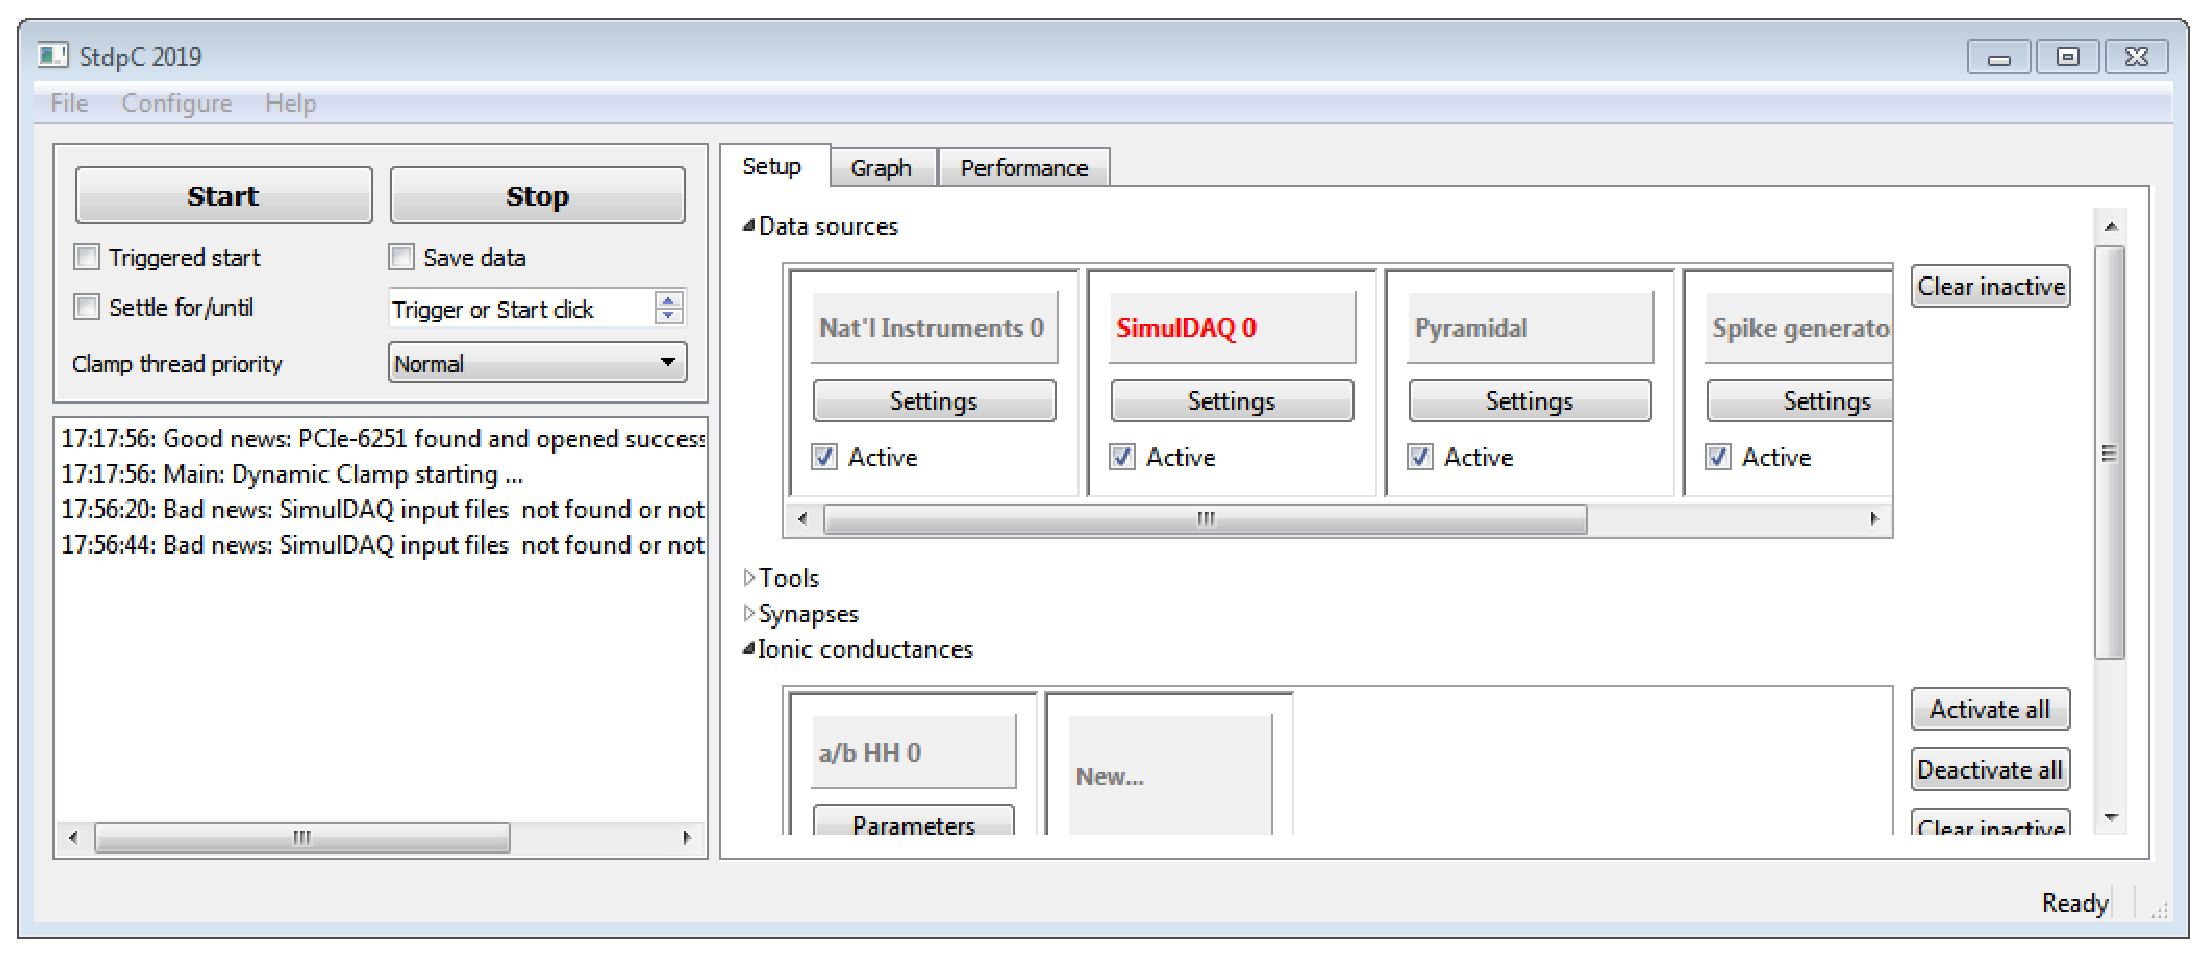
\includegraphics[width=\textwidth]{main}
}
\vspace*{0.5cm}

The main control panel contains different blocks of control for the
different functions of the software -- simulating synapses (synapse
control block; 1), simulating ionic conductances (Hodgkin-Huxley (HH)
type conductances; HH control block; 2), simulating presynaptic
activity (spike generator block; 3) and displaying data (data
displays; for debugging only; 4). The control blocks are front-ends to
more detailed control dialogs. There is a message window in the upper
left part of the panel that shows system messages. These messages can
be saved for future reference. They are also automatically written to
a local file ``StdpC\_last.log''.


\subsection{Configuration of the Hardware and Control of the Program}

\parbox[b]{0.35\textwidth}{
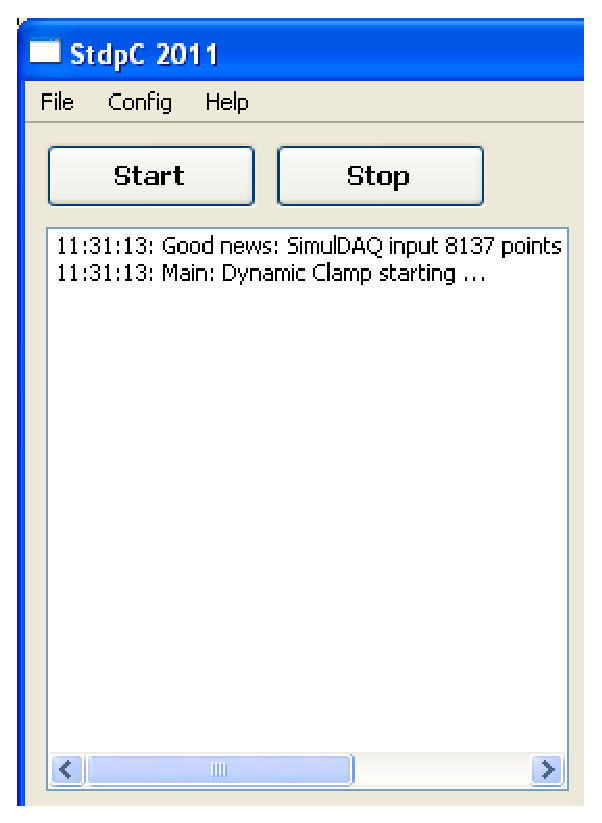
\includegraphics[scale=0.5]{mainBlock}
} \hfill
\parbox[b]{0.64\textwidth}{ Once StdpC is started, the last known hardware
  configuration is loaded (from a local file named
  ``StdpC.conf''). Other parameters are initialized with standard
  values that are pre-compiled into the software. The message window
  will show a message whether the chosen hardware was successfully
  initialized (which was not the case in the example shown on the left).

Failing hardware initialization can have several causes: \\[-0.2cm]
\begin{myenum}
\item If using the DigiData 1200(A): \\
StdpCs default address for the board is 0x320 (hexadecimal), which
is the default address of the board, but the specific board can have been
configured to use another range of addresses. Possible values are 0x340,
0x360, 0x380, 0x3A0, 0x3C0, etc. Make sure that the correct address is
entered in the ``DAQ'' dialog.
\end{myenum}
} \\

\begin{myenum}
\addtocounter{enumi}{1}
\item If using a National Instruments board: \\
Make sure that NIDAQmx is installed and the board is working properly
(using the NI Automation explorer). Make sure your device is in the
list of devices that support NIDAQmx (as opposed to the older devices
supporting ``old style'' NIDAQ / NIDAQ legacy only.
\item I you are running with simulated data acquisition: \\
Make sure that you have a correctly formatted input file for the
membrane potential of cells and that the filename in the ``DAQ''
dialog points to the right location of this file. Also make sure that the
location the output filename points to is writable to you.
\end{myenum}

The remaining controls are the ``start'' and the ``stop'' button.  The
``start'' button initiates the start of dynamic clamp cycles. In
particular, pressing this button will stop a running dynamic clamp
thread, load the settings from (almost) all dialogs into memory, and
start a the dynamic clamp thread again with the new settings. The
dynamic clamp thread will then run until stopped by pressing the
``stop'' button.

The data acquisition hardware can be chosen in the combo box on the
top. Note that the software that has been compiled with support for
the NIDAQmx libraries will not run if these are not installed {\em
  even if a different device is chosen}. The specific hardware
settings can be adjusted in the ``DAQ'' dialog int the ``Config''
menu of the main menu bar.

The choice of hardware, its settings and the settings for input and
output channels are the only exception to the rule that changes only
apply after a restart of the dynamic clamp thread (by pressing the ``start''
button).

Other general control elements can be found in the menus of the main
menu bar. 
\begin{myitem}
\item ``File'' menu:
\
\begin{itemize}
\item[-] ``Load Protocol'': Load parameter settings from a previous
  session. The standard filename extension for these is ``cpr'',
  albeit the settings are saved in it in plain ASCII format.
\item[-] ``Save Protocol'': Save the current parameter settings into a
  file for later use or documentation.
 \item[-] ``Load Script'': Load a script for experiment
   automation. Scripting is described in section \ref{scriptsect}.
\item[-] ``Unload Script'': Remove a script from memory and use StdpC
  interactively.
\item[-] ``Export Log'': Export the contents od the message box to a
  file.
\item[-] ``Clear Log'': Remove the message box contents.
\item[-] ``Exit'': Quit StdpC.
\end{itemize}
\item ``Config'' menu:
\begin{itemize}
\item[-] ``DAQ'': Controls for the properties of the data acquisition
  hardware. This will show a dialog window that is specific to the
  chosen hardware. For an example for a simulated DAQ, see below.
\item[-] ``Input Channels'': Brings up a dialog to change settings for
  the analog input channels, see below for more details.
\item[-] ``Output channels'': Brings up a corresponding dialog for the
  output channels, see below.
\end{itemize}
\item ``Help'': Offers a one-line description about StdpC. 
\end{myitem}

%% new Address: Button used to change the hardware address of the Digidata
%% board. A new hexadecimal value should be typed in the corresponding field
%% before pressing this button. When the board is found the Status Window will
%% display the respective message.
%% \item AMP X: field that indicates the gain factor of the microelectrode
%% amplifier connected to the channel X. To change the default value
%% click in the field containing the address and edit the value using the
%% keyboard.
%% \item ADC X: configures the input gain of the ADC channel X in the Digidata
%% board. It is related to the precision of the A/D conversion and should be
%% selected as big as possible. Allowed values for this parameter are: 8, 4, 2,
%% 1, respectively corresponding to the ranges of input voltages -1.25V to
%% +1.25V, -2.5V to +2.5V, -5.0V to + 5.0V, and -10.0V to +10.0V.
%% \item mV/nA: correspond to the calibration of the current input command
%%   voltage in the microelectrode amplifiers in mV/nA for each channel. Since
%%   the range of the current voltage command output is -10V to +10V, one can
%%   select a higher ratio mv/nA and use a divider to match it to the input of
%%   the microelectrode amplifier, increasing the precision of the current
%%   generation.
%% \item The output channel 1 is either used for clamping in which case the
%%   settings are as for channel 0 or it outputs the membrane voltage of the
%%   spike generator if it is used. Then, the setting CN\_Vm =$>$ CH1 sets a gain
%%   factor for the output of the spike generator membrane voltage.
%% \item Write State: Upon pressing this button the state of the StdpC, {\em
%%   i.e.} the values of {\em all} prameters and {\em all} status buttons is
%%   saved in a file (typically with extension ``.set'').
%% \item Read State: Upon pressing this button a file dialog appears and one can
%%   choose a previously ``.set'' file to be loaded. This will update {\em all}
%%   parameters and status buttons.
%% \item Exit: Exits the StdpC program.


\subsection{Electrical synapses}

\noindent
\parbox{\textwidth}{
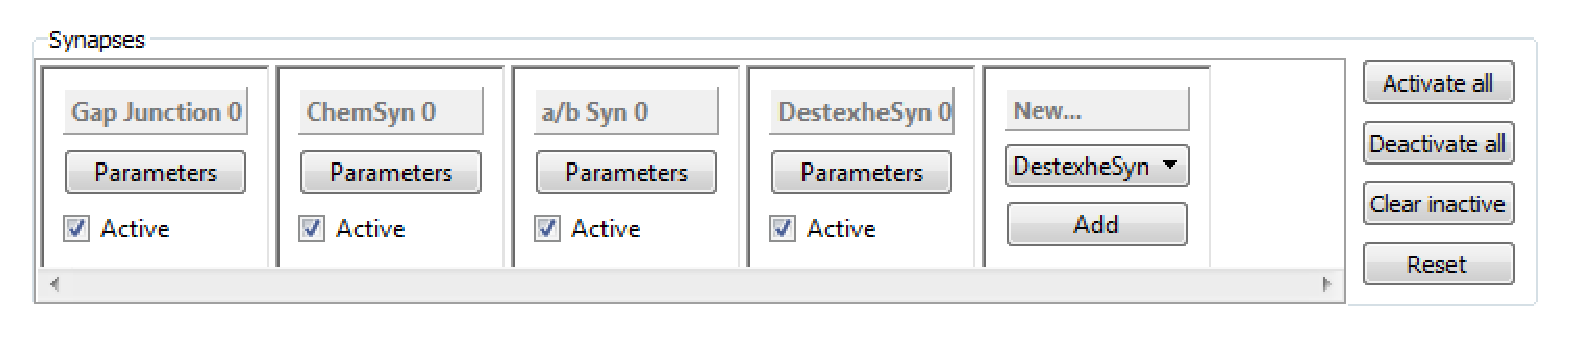
\includegraphics[scale=0.5]{synapseBlock}
} \\[0.2cm]

Each subunit in the synapses block can be configured to be a
chemical or an electrical synapse (gap junction). Clicking the
``Parameters'' button will open a control panel that allows to change
propertis of the synapse. \\

\noindent
\parbox{0.4\textwidth}{
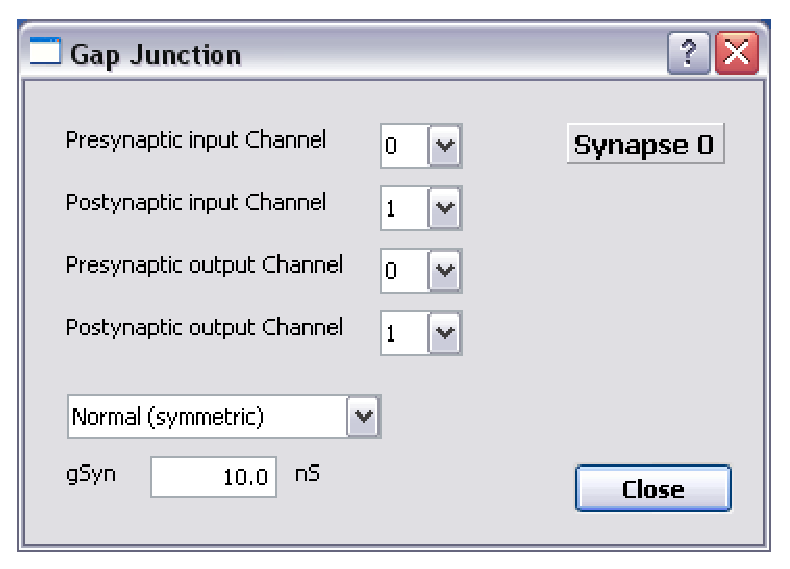
\includegraphics[scale=0.5]{gapJunctionDialog}
}
\hfill
\parbox{0.55\textwidth}{
If configured as an electrical synapse the control window on the left
will appear. 

The currents $I_{\text{pre}}$ and $I_{\text{post}}$ to be injected
into the pre- and post-synaptic cells, respectively, are calculated
according to:
\begin{align}
  I_{\text{post}}(t) &= g_{\text{Syn}} [V_{\text{pre}}(t) - V_{\text{post}}(t)],  \\
  \text{and} \quad I_{\text{pre}}(t) &= -I_{\text{post}}(t), 
\end{align}
where $V_{\text{pre}}(t)$ and $V_{\text{post}}(t)$ are the membrane
potential of the two cells. If the gap junction is chosen as
rectifying, $I_x (t)= 0$ if $V_{\text{pre}}(t) < V_{\text{post}}(t)$.
} \\[0.2cm]
 The control elements are
\begin{myitem}
\item Presynaptic input channel: Combo to choose the input channel
  that contains the membrane potential of the presynaptic cell (SP= spike
  generator) 
\item Postynaptic input channel: Combo to choose the input channel
  that contains the membrane potential of the postynaptic cell 
\item Presynaptic output channel: Combo to choose the output channel
  that will contain the current command for the presynaptic cell. 
\item Postynaptic output channel: Combo to choose the output channel
  fot the current command intended for the postsynaptic cell.
\item Type combo: Choose whether the gap junction is ordinary (the
  current can flow from the pre-synaptic cell to the postsynaptic cell
  an vice versa; both cells have perfectly symmetrical roles in this
  case) or rectifying (positive current can only from the presynaptic
  cell to the possynaptic cell but not in the other direction). 
\item gSyn: Conductance of the gap junction in nS.  
\end{myitem}

\subsection{Chemical Synapses}
If the type of synapse is chemical, the control dialog of a chemical
synapse is displayed on pressing ``Parameters''. The current to be
injected into the postsynaptic cell, $I_{\text{post}}$, is calculated
in each dynamic clamp cycle using a first order kinetics model of the
release of neurotransmitter \cite{Destexhe1994} and an additional
inactivation term, $h(t)$, to simulate short term depression:
\begin{align}
  I_{\text{post}} = g_{\text{Syn}} \, S(t) \, h(t) [V_{\text{Syn}} -
    V_{\text{post}}(t)],
\end{align}
where the instantaneous activation, S(t), and inactivation, h(t), terms are
given by the differential equations
\begin{align}
(1-S_\infty(V_{\text{pre}})) \tau_{\text{Syn}} \frac{dS(t)}{dt} &=
(S_\infty(V_{\text{pre}}) - S(t)) \\ \tau_h \frac{dh(t)}{dt} &=
h_\infty(V_{\text{pre}}) - h(t),
\end{align}
where
\begin{align}
S_\infty(V_{\text{pre}}) &= \left\{
\begin{array}{ll}
  \tanh\left[\frac{V_x(t) - V_{\text{Thresh}}}{V_{\text{Slope}}}
    \right] & \text{if } V_{\text{pre}} > V_{\text{Thresh}} \\ 0 &
  \text{otherwise}
  \end{array}
\right. \\ 
%
h_\infty(V_{\text{pre}})&=
\frac{A}{1+\exp\left(\frac{V_{\text{pre}} -
    V_{\text{Thresh}}}{V_{\text{Slope}}}\right)}, \\  
\tau_h(V_{\text{pre}})&= \tau_{0} -
\frac{A_\tau}{1+\exp\left(\frac{V_{\text{pre}} -
    V_{\text{Thresh},\tau}}{V_{\text{Slope},\tau}} \right)}
\end{align}                                              
  The controls in the paramter dialog for the chemical synapse are
  \begin{myitem}
  \item Presynaptic Channel: Combo box to choose the input channel
    that contains the membrane potential of the presynaptic cell (SP = spike
    generator) 
  \item Postynaptic Channel: Combo box that contains the membrane
    potential of the postynaptic cell
\item Output Channel: The output channel to which the current command
  for the synapse will be added
\end{myitem}
``Standard'':
\begin{myitem}
  \item gSyn: The maximal conductance $g_{\text{syn}}$ of the synapse in nS. 
  \item VSyn: The reversal potential $V_{\text{Syn}}$ in mV. 
\item tauSyn: The characteristic time constant $\tau_{\text{Syn}}$ of
  the synapse in ms.  
\item VThresh: The threshold  potential $V_{\text{Thresh}}$ for the
  release of neurotransmitter in mV.  
\item VSlope: The ``slope'' parameter $V_{\text{Slope}}$ of the
  activation curve in mV.  
  \end{myitem}
                                                          
\noindent
\parbox[b]{0.48\textwidth}{
  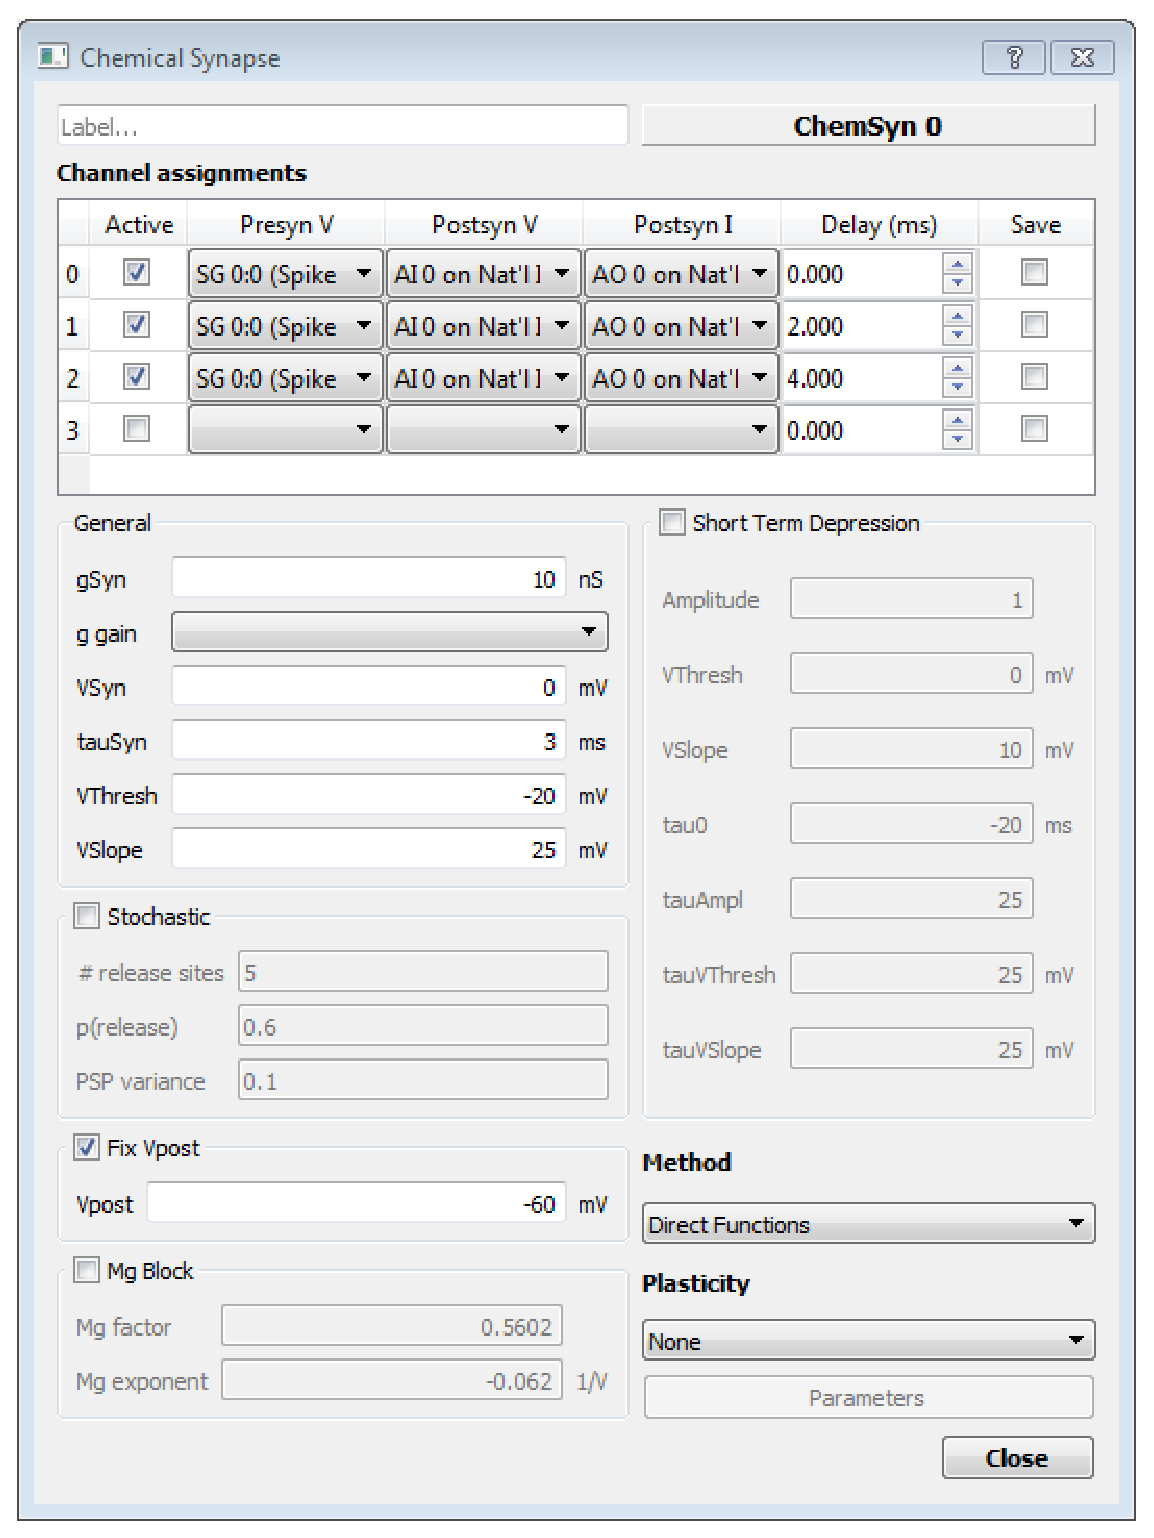
\includegraphics[scale=0.5]{chemicalDialog}
}
\hfill
\parbox[b]{0.5\textwidth}{
``Short Term Depression'':
\begin{myitem}
\item Combo box to switch this mechanism on or off
\item Amplitude: The amplitude of the $h(t)$ depression
  variable. Typically set to 1 (so that $h$ varies between $0$ and
  $1$). This was previously used to switch short term depression on or
  off and remains for historical reasons.
\item VThresh: The threshold potential $V_{\text{Thresh},\tau}$ for
  the activation of $h$ in mV.  
\item VSlope: The ``slope'' parameter of the depression activation
  curve in mV. 
\item tau0, tauAmpl, tauVThresh, and tauVSlope: Parameters $\tau_0$,
  $A_\tau$, $V_{\text{Thresh},\tau}$ and $V_{\text{Slope},\tau}$ for
  the voltage-dependent characteristic time $\tau_h$ of short term depression.
\item The plasticity combo box allows to choose whether the synapse is
  subject to long term plasticity and according to which model the
  plasticity is determined.\end{myitem}
} \\[0.2cm]
%
\mbox{}\hfill\parbox[t]{0.95\textwidth}{ For ``Spike STDP'' a spike-timing based
  rule is applied according to the parameters defined in the
  corresponding control panel that appears upon clicking the
  ``Parameters'' button. If ``ODE STDP'' is chosen, the synaptic
  plasticity is implemented according to the ordinary differential
  equation (ODE) description in \cite{Abarbanel2002}. Prameters again
  are adjusted in the separate panel that appears after pressing
  ``Parameters''.
} \\\mbox{}
\subsection{Spike Timing Dependent Plasticity}
As described above, synapses can be equipped with a form of Spike
Timing Dependent Plasticity (STDP).
The typical way of implementation, denoted as ``Spike STDP'',
is to detect spikes in the pre- and postsynaptic cells and 
define 
  \begin{align}
    \Delta g= \pm A_{\pm} \left(\frac{|\Delta t -
      \tau_{\text{Shift}}|}{\tau_{\pm}}\right)^q
    \exp\left(-\frac{|\Delta t -
      \tau_{\text{Shift}}|}{\tau_{\pm}}\right) .
  \end{align}
$\Delta g$ is then added to the ``raw'' synaptic conductance
$g_{\text{raw}}$ whenever a pre- or postsynaptic spike occurs. Note
that for correct function, spike detection needs to be switched on
for the pre- and postsynaptic input channels (see input channel
dialog). The synaptic conductance $g_{\text{Syn}}$ is then
determined from $g_{\text{raw}}$ through a sigmoid filter
\begin{align}
  g= g_{\text{max}} \tanh\left(\frac{g_{raw} -
    g_{\text{Mid}}}{g_{\text{Slope}}}\right) 
\end{align}
to avoid problems of ``run-away'' potentiation.

\noindent
\parbox{0.45\textwidth}{
  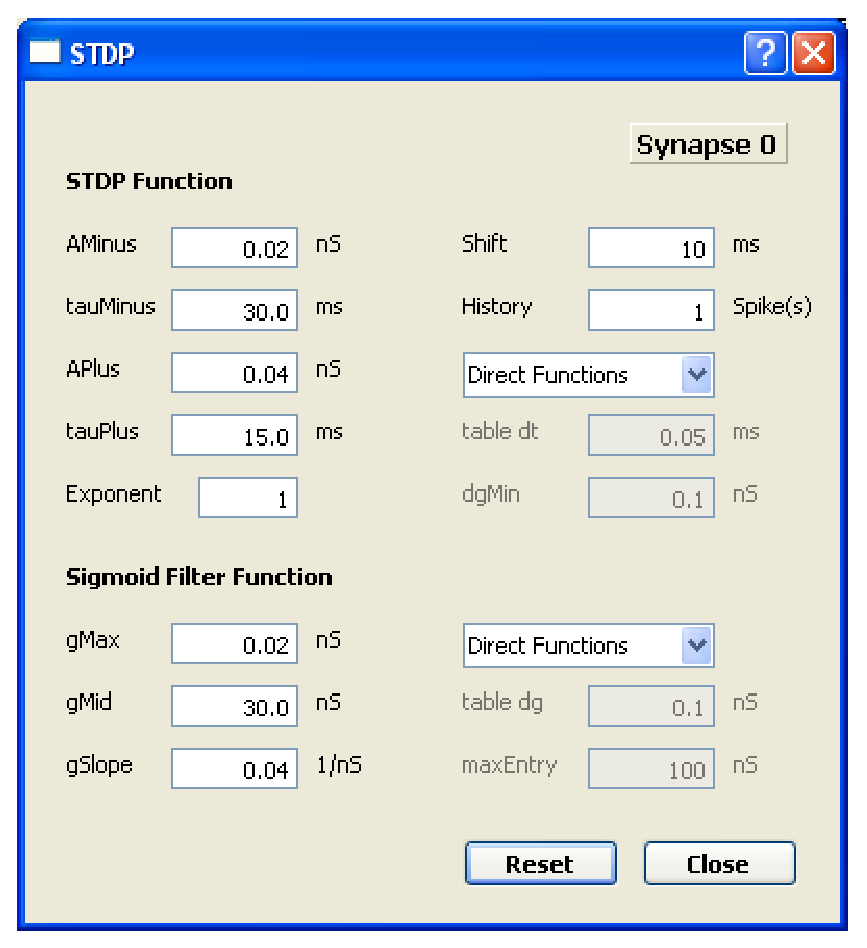
\includegraphics[scale=0.5]{StdpDialog}
}
\hfill
\parbox{0.5\textwidth}{
The control parameters are: \\
``STDP Function''
\begin{myitem}
\item AMinus: The amplitude $A_-$ of the negative (left) part of the STDP curve.
\item tauMinus: The time scale $\tau_-$ (locus of the extremum) of the negative
  (left) part of the STDP curve.
\item APlus: The amplitude $A_+$ of the positive (right) part of the
  STDP curve.
\item tauPlus: The time scale $\tau_+$ (locus of the extremum) of the
  positive (right) part of the STDP curve.
\item Exponent: The exponent $q$ of the polynomial factor in the STDP
  curve. 
\item Shift: The offset $\tau_{\text{Shift}}$ of the STDP curve on the
  $\Delta t$ axis. 
\end{myitem}
}\\
\begin{myitem}
\item History: The number of spikes to be considered in the other
  neuron if a spike occurs in a given neuron. For example, if set to
  $1$ and a spike occurs in the postsynaptic neuron, the change 
  $\Delta g$ will only be calculated and applied for the last spike
  that occurred in the presynaptic neuron. If it was $2$ it would be
  calculated for the last and the next to last spike in the
  presynaptic neuron.
\item The method combo box allows to choose whether the STDP function is
  calculated directly with the approriate C functions when needed or
  whether it is tabled up front and this lookup-table is being used.
\item table dt: The time step in the lookup table.
\item dgMin: The minimum value for $\Delta g$ that should be in the
  table. This determines how far to the left and right the table
  covers the STDP curve.
\end{myitem}
``Sigmoid Filter Function''
\begin{myitem}
\item gMax: The maximal $g_{\text{Syn}}$ allowed.
\item gMid: The midpoint $g_{\text{Mid}}$ of the filter.
\item gSlope: The ``slope'' parameter $g_{\text{slope}}$ of the sigmoid filter. 
\item The method combo allowing the choice between direct calculation
  or lookup tables for the filter function.
\item table dg: The stepping in terms of $g_{\text{raw}}$ of the
  lookup table.
\item maxEntry: The maximal $g_{\text{raw}}$ entry in the table.
\end{myitem}


Alternatively the synaptic strength is governed by a set of differential
equations according to the model of synaptic plasticity in
\cite{Abarbanel2002}. In this case, the maximal synaptic conductance
$g_{\text{Syn}}$ is subject to a differential equation system
\begin{align}
\frac{dP}{dt} = v_{\text{pre}} - \beta_P P \\
\frac{dD}{dt} = v_{\text{post}} - \beta_D D \\
\frac{dg_{\text{raw}}}{dt} = \gamma (P D^\eta - D P^\eta).
\end{align}
The normalized voltages $v_x$ are derived from the measured potentials
$V_x$ through capped linear filters
\begin{align}
v_{\text{pre}} = \left\{ \begin{array}{ll}
0 & V_{\text{pre}} < V_{P,\text{min}} \\
\frac{V_{\text{pre}}-V_{P, \text{min}}}{V_{P, \text{max}}-V_{P,
    \text{min}}} & V_{P, \text{min}}\leq V_{\text{pre}} \leq V_{P,
  \text{max}} \\
1 & V_{P, \text{max}} < V_{\text{pre}} 
\end{array} \right.
\end{align}
and accordingly for $v_{\text{post}}$,
\begin{align}
v_{\text{post}} = \left\{ \begin{array}{ll}
0 & V_{\text{post}} < V_{D,\text{min}} \\
\frac{V_{\text{post}}-V_{D, \text{min}}}{V_{D, \text{max}}-V_{D,
    \text{min}}} & V_{D, \text{min}}\leq V_{\text{post}} \leq V_{D,
  \text{max}} \\
1 & V_{D, \text{max}} < V_{\text{post}} 
\end{array} \right.
\end{align}
\vspace*{0.3cm}

\noindent
\parbox{0.48\textwidth}{
  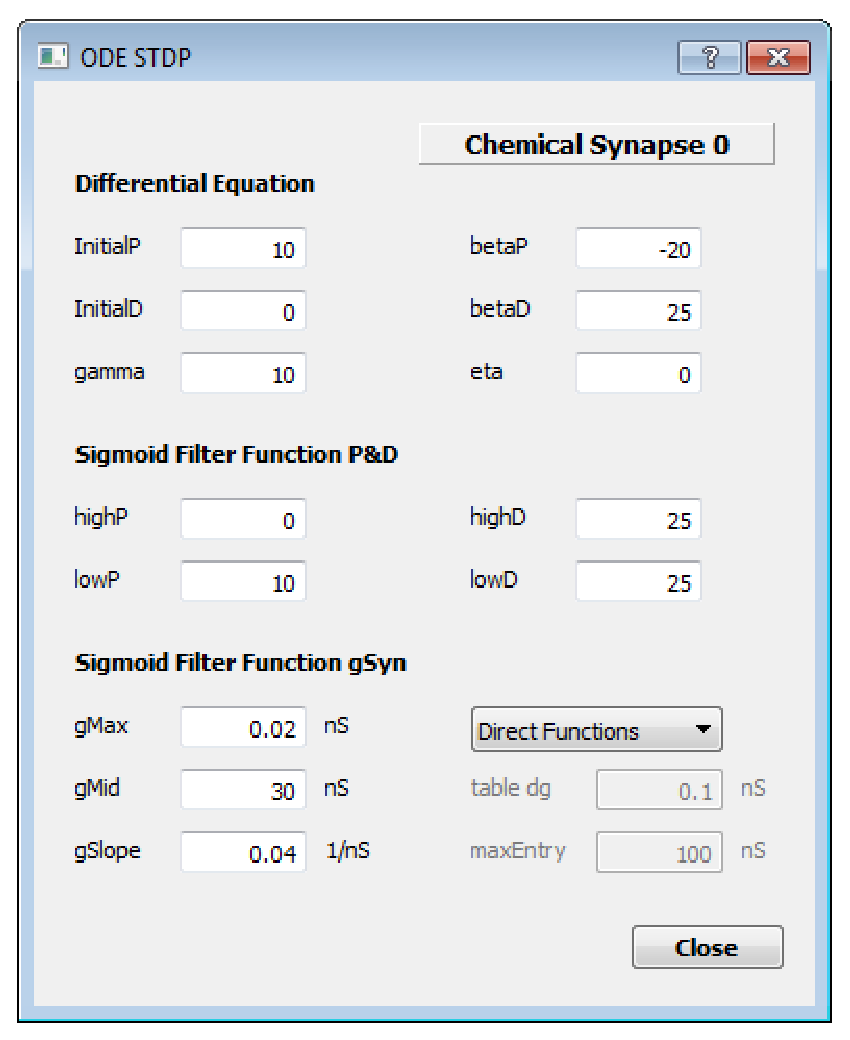
\includegraphics[scale=0.5]{odeStdpDialog} 
}
\hfill
\parbox{0.5\textwidth}{
The control parameters for ODE based STDP are: \\
``Differential Equation''
\begin{myitem}
\item InitialP: Initial value for the ``potentiation variable'' $P$
\item InitialD: Initial value for the ``depression variable'' $D$
\item gamma: Exponent $\gamma$
\item betaP: Rate of decay $\beta_P$ of $P$ in 1/ms= kHz.
\item betaD: Rate of decay $\beta_D$ of $D$ in 1/ms= kHz.
\item eta: Rate of change of $g_{\text{raw}}$ in nS/ms.
\end{myitem}
``Sigmoid Filter Function P \& D''
\begin{myitem}
\item highP: The upper limit $V_{P, \text{max}}$ of the $P$ filter 
\item lowP: The lower limit $V_{P, \text{min}}$ of the $P$ filter 
\item highD: The upper limit $V_{D, \text{max}}$ of the $D$ filter
\item lowD: The lower limit $V_{D, \text{min}}$ of the $D$ filter
\end{myitem}
}\\

``Sigmoid Filter Function gSyn''
\begin{myitem}
\item gMax: The maximal allowed value for $g_{\text{Syn}}$.
\item gMid: The mid point of the sigmoid filter gor $g_{\text{Syn}}$
\item gSlope: The ``slope'' parameter of the sigmoid filter function
  for $g_{\text{Syn}}$.
\item The method combo allows to switch between direct evaluation of
  the filter or the use of a lookup table
\item table dg: The step size in the lookup table
\item maxEntry: The maximum of $g_{\text{raw}}$ for which table
  entries are generated.
\end{myitem}  
\subsection{Hodgkin-Huxley Type Conductances}

\parbox{\textwidth}{
  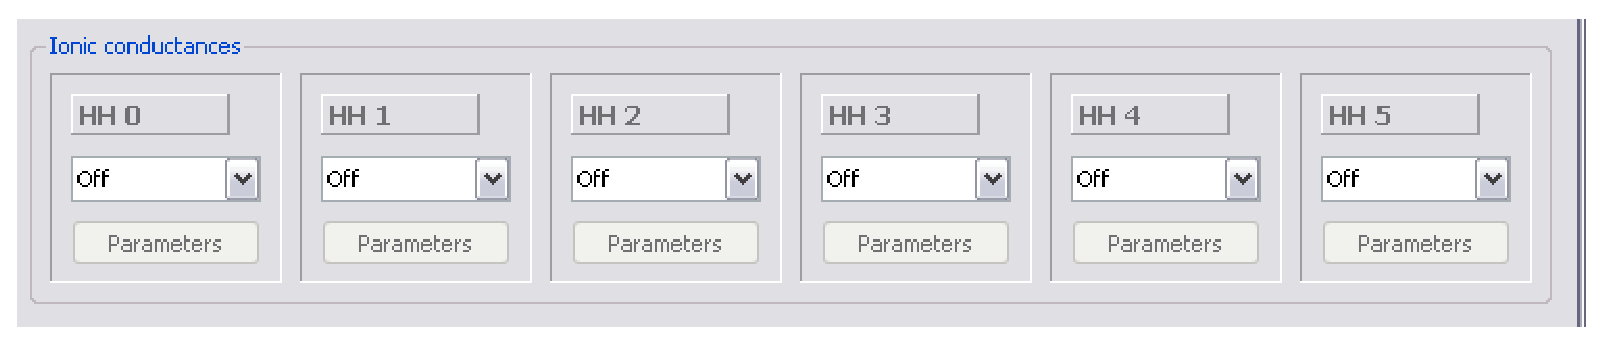
\includegraphics[scale=0.5]{HHBlock}
} \\[0.2cm]
 
StdpC can inject up to six Hodgkin-Huxley type ionic conductances into
cells. The six conductances can be inserted into a single cell
or into several cells in any desired combination. The control blocks
of Hodgkin- Huxley type conductances allow to choose two different
types for the description.

For the ``m/h/tau'' description, the current $I_{HH}$ to be injected
into a cell with membrane potential V(t) is calculated according to
\begin{align}
  I_{HH}(t) = g_{\text{Max}} m(t)^p h(t)^q (V_{\text{rev}}-V(t)),
\end{align}
where $m$ and $h$ are modeled as
\begin{align}
  \tau_m \frac{dm}{dt} &= m_\infty(V)-m , \\
  \tau_h \frac{dh}{dt} &= h_\infty(V)- h, 
\end{align}
with steady state values
\begin{align}
  m_\infty &= \frac{1}{1+\exp \left(\frac{V - V_m}{s_m}
  \right)}, \\
  h_\infty &= \frac{1}{1+\exp \left(\frac{V - V_h}{s_h}
  \right)}, 
\end{align}
and time scales 
\begin{align}
  \tau_m &= \tau_{0,m} - 
  \frac{A_{\tau,m}}{1+\exp\left(\frac{V-V_{\tau,m}}{s_{\tau,m}}\right)}, \\
  \tau_h &= \tau_{0,h} - 
  \frac{A_{\tau,h}}{1+\exp\left(\frac{V-V_{\tau,h}}{s_{\tau,h}}\right)}, 
\end{align}
  
\noindent
\parbox{0.48\textwidth}{
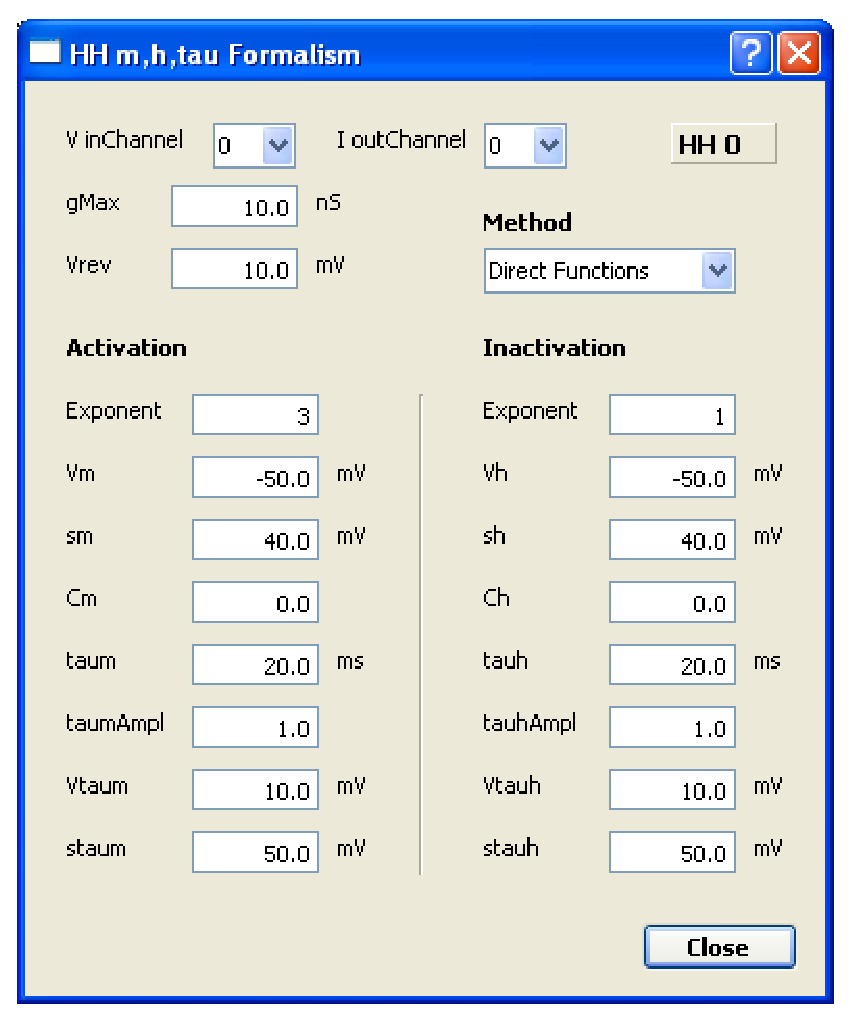
\includegraphics[scale= 0.5]{mhtauDialog}
} 
\hfill
\parbox{0.5\textwidth}{
Control parameters of the ionic conductances in the m/h/tau formalism
are:
\begin{myitem}
\item V in Channel: The input channel that contains the membrane
  potential of the cell the conductance is injected into
\item I out Channel: The output channel to which the current command
  for the inserted ionic conductance will be added
\item gMax: The maximal conductance $g_{\text{Max}}$ of the inserted
  channel
\item Vrev: The reversal potential $V_{\text{rev}}$ of the inserted
  channel
\item Method: The combo box allows to choose between direct evaluation of C
  functions or a pre-calculated lookup table.
\end{myitem}
} \\[0.2cm]

\noindent
``Activation''
\begin{myitem}
\item Exponent: The exponent $p$ in the current equation
\item Vm: The activation potential $V_m$
\item sm: The width $s_m$ of the activation function
\item Cm: The offset parameter $C_m$ for persistent currents 
\item taum: The minimal time scale $\tau_{0,m}$ for $\tau_m$.
\item taumAmpl: The range (Amplitude) $A_{\tau\,m}$ for the time scale $\tau_m$.
\item Vtaum: The mid point $V_{\tau,m}$ for the time scale sigmoid function.
\item staum: The ``slope'' parameter $s_{\tau,m}$ for the time scale
sigmoid function  
\end{myitem}
``Inactivation''
\begin{myitem}
\item Exponent: The exponent $q$ in the current equation
\item Vh: The inactivation potential $V_h$
\item sh: The width $s_h$ of the inactivation function
\item Ch: The offset parameter $C_h$ for persistently inactivated currents 
\item tauh: The minimal time scale $\tau_{0,h}$ for $\tau_h$.
\item tauhAmpl: The range (Amplitude) $A_{\tau,h}$ for the time scale $\tau_h$.
\item Vtauh: The mid point $V_{\tau,h}$ for the time scale sigmoid function.
\item stauh: The ``slope'' parameter $s_{\tau,h}$ for the time scale
sigmoid function.  
\end{myitem}

\noindent
Alternatively, the ionic conductances can be described in a
$\alpha$/$\beta$ formalism, where
\begin{align}
I_{\text{Syn}}= g_{\text{Max}} m^p h^q (V_{\text{rev}}-V) \\
\frac{dm}{dt}= \alpha_m (1-m) - \beta m \\
\alpha_m= k_{\alpha,m} F_{\alpha,m}\left(\frac{V-V_{\alpha,n}}{s_{\alpha,m}}
\right) \\
\beta_m= k_{\beta,m} F_{\beta,m}\left(\frac{V-V_{\beta,n}}{s_{\beta,m}}
\right) \\
\frac{dh}{dt}= \alpha_h (1 - h) - \beta_h h \\
\alpha_h= k_{\alpha,h} F_{\alpha,h}\left(\frac{V-V_{\alpha,n}}{s_{\alpha,h}}
\right) \\
\beta_h= k_{\beta,h} F_{\beta,h}\left(\frac{V-V_{\beta,n}}{s_{\beta,h}}
\right).
\end{align}
The ``activation''/''inactivation'' functions $F_{\bullet , \bullet}$ can
be chosen from three choices,
\begin{align}
F_1(x)= \frac{x}{\exp(x)-1} \\
F_2(x)= \exp(x) \\
F_3(x)= \frac{1}{1+\exp(x)}.
\end{align}
Note, that this formalism allows to implement, for example, the classic
neuron model by Traub and Miles \cite{Traub1991}. \\

\noindent
\parbox{0.58\textwidth}{
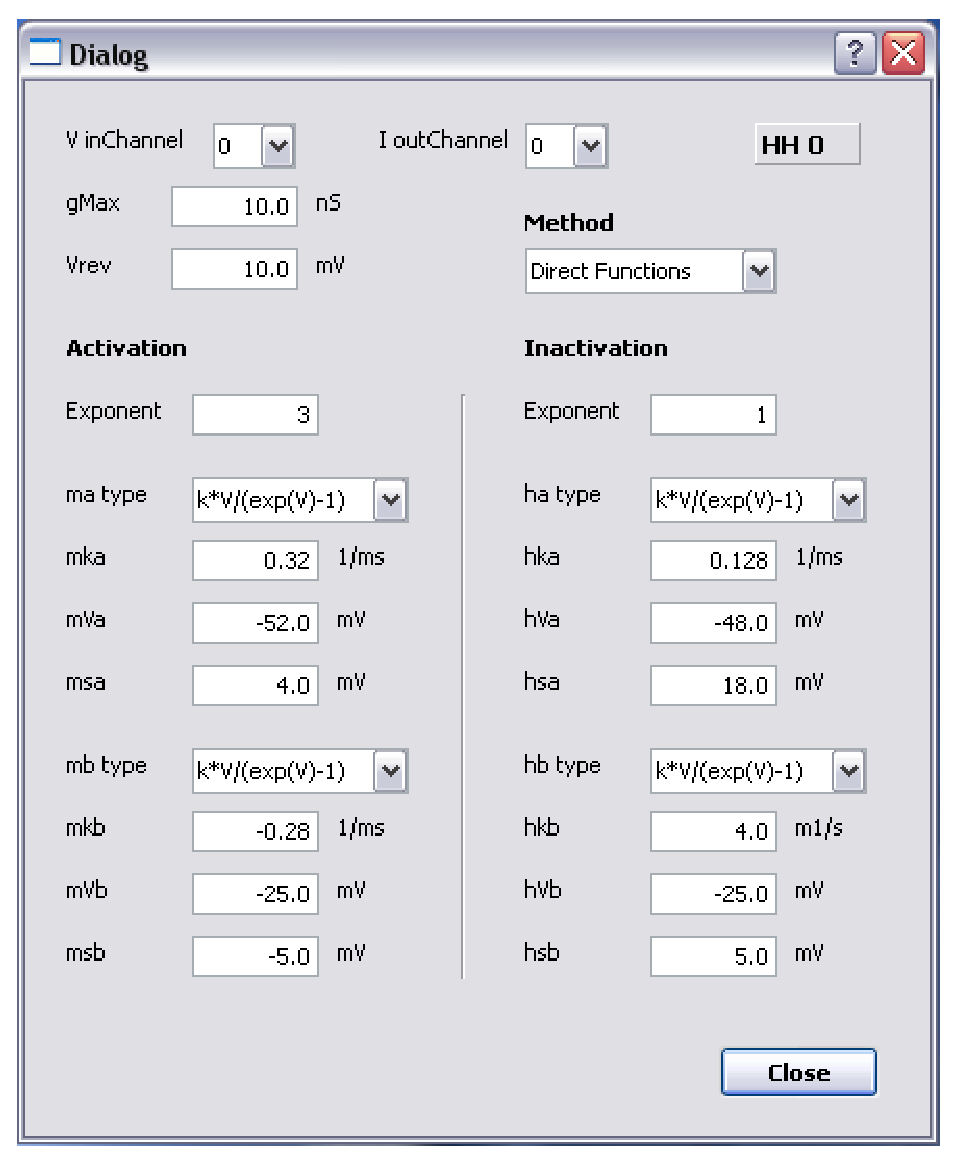
\includegraphics[scale= 0.5]{alphaBetaDialog}
}
\hfill
\parbox{0.4\textwidth}{
The control parameters are
\begin{myitem}
\item V in Channel: The input channel that contains the membrane
  potential of the cell the conductance is injected into
\item I out Channel: The output channel to which the current command
  for the inserted ionic conductance will be added
\item gMax: The maximal conductance $g_{\text{Max}}$ of the inserted
  channel
\item Vrev: The reversal potential $V_{\text{rev}}$ of the inserted
  channel
\item Method: The combo box allows to choose between direct evaluation of C
  functions or a pre-calculated lookup table.
\end{myitem}
} \\[0.2cm]

\noindent
``Activation''
\begin{myitem}
\item Exponent: The exponent $p$ in the current equation
\item ma type: The choice of the functional form for $F_{\alpha,m}$.
\item mka: Rate parameter $k_{\alpha,m}$ for the rise of $m$
\item mVa: The midpoint $V_{\alpha,m}$ for the sigmoid function
  for $\alpha_m$ 
\item msa: The ``slope'' parameter $s_{\alpha,m}$ for the sigmoid function
  for $\alpha_m$
\item mb type: The choice of the functional form for $F_{\beta,m}$.
\item mkb: Rate parameter $k_{\beta,m}$ for the decay of $m$
\item mVb: The midpoint $V_{\beta,m}$ for the sigmoid function
  for $\beta_m$ 
\item msb: The ``slope'' parameter $s_{\beta,m}$ for the sigmoid function
  for $\beta_m$
\end{myitem}
``Inactivation''
\begin{myitem}
\item Exponent: The exponent $q$ in the current equation
\item ha type: The choice of the functional form for $F_{\alpha,h}$.
\item hka: Rate parameter $k_{\alpha,h}$ for the rise of $h$
\item hVa: The midpoint $V_{\alpha,h}$ for the sigmoid function
  for $\alpha_h$ 
\item hsa: The ``slope'' parameter $s_{\alpha,h}$ for the sigmoid function
  for $\alpha_h$
\item hb type: The choice of the functional form for $F_{\beta,h}$.
\item hkb: Rate parameter $k_{\beta,h}$ for the decay of $h$
\item hVb: The midpoint $V_{\beta,h}$ for the sigmoid function
  for $\beta_h$ 
\item hsb: The ``slope'' parameter $s_{\beta,h}$ for the sigmoid function
  for $\beta_h$
\end{myitem}


\subsection{Spike generator}
The spike generator unit can replace a presynaptic cell. It can
operate in several very different modes. When its input are spike
timings, the spikes have a
pre-defined form. Alternatively it can replay a voltage waveform from
a file directly. The spike time information can either be explicit
spike times from a file, spike patterns (bursts) specified in a file,
or a spike pattern defined explicitly through the graphical interface.
The pattern options can be combined with burst detection, in which
each spike pattern is triggered by a detected thershold event in
another (measured) neuron.

The control elements for the spike generator are
\begin{myitem}
\item The ``Spike Method'' combo allows to choose the type of operating
  method -- explicit spike times from the GUI, spike times from a file
  (that includes explicit times if burst detection is not enabled, or
  burst patterns if it is), and replay of a voltage waveform from a
  file.
\item The method combo allows to choose for the use of functions or
  lookup tables.
\end{myitem}

\noindent
\parbox{0.48\textwidth}{
    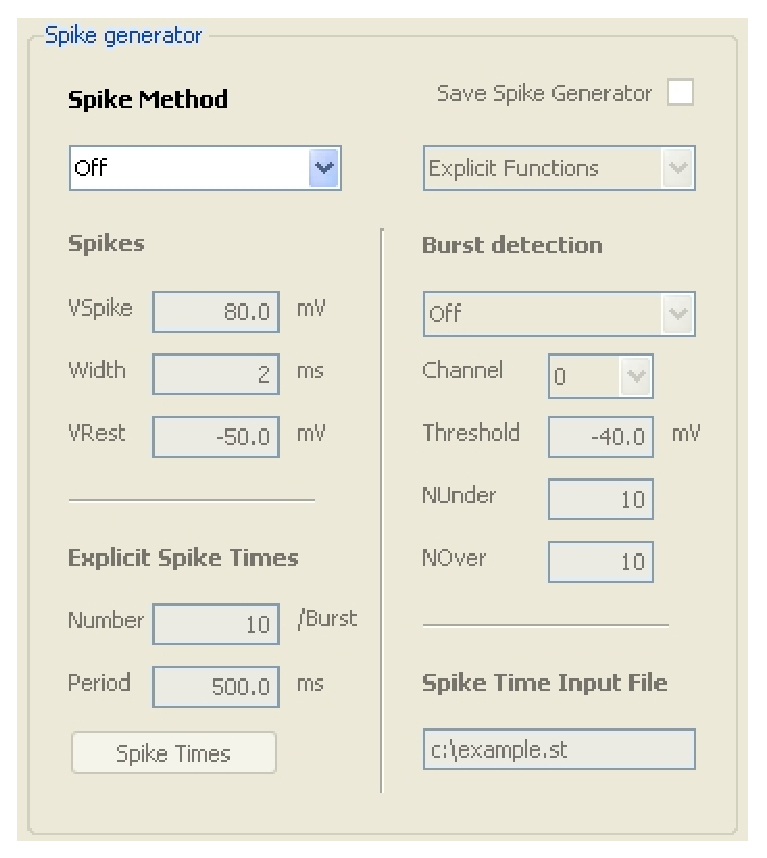
\includegraphics[scale=0.5]{spikeGenBlock}
}
\hfill
\parbox{0.5\textwidth}{
``Spikes''
\begin{myitem}
\item VSpike: The amplitude of the spikes generated
\item Width: The width of spikes in ms
\item VRest: Th resting potential from which the spikes depart
\end{myitem}
``Explicit Spike Times'' \\
If this method was chosen, the parameters are
\begin{myitem}
\item Number: The number of spikes in the pattern (burst)
\item Period: The period with which to repeat the spike pattern
  periodically 
\item The ``Spike Times'' button will make the window visible, in
  which explicit spike times can be entered
\end{myitem}
}\\[0.2cm]

\noindent
\parbox{0.48\textwidth}{
    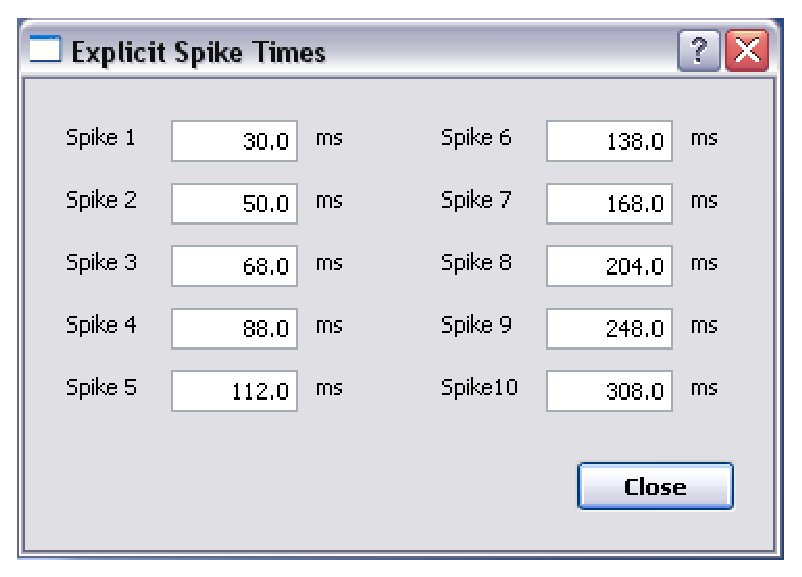
\includegraphics[scale=0.5]{spikeTimeDialog}
}
\hfill
\parbox{0.5\textwidth}{
``Burst detection''
\begin{myitem}
\item The transition combo allows to choose whether to trigger an
  event for low to high or high to low transitions through a threshold
  value
\item Channel: The input channel on which to detect events
\end{myitem}
}
\begin{myitem} 
\item Threshold: The trigger threshold for event detection. For
  low$\rightarrow$high detection, an event
  is triggered whenever NUnder measurements were below threshold and
  afterwards NOver measurements were above. Note that for noisy
  signals it may be  necessary to increase both numbers for reliable
  detection. The events below and above are not required to be
  contiguous in the current implementation.
\item NUnder: see ``Threshold'' above.
\item NOver: see ``Threshold'' above.
\end{myitem}
``Spike Time Input File''
\begin{myitem}
\item The input filename for the file that contains the spike time
  information. If burst detection is off, the file should contain one
  clear text column containing times in seconds when spikes shall
  occur.
If burst detection is on, StdpC 2007 expects descriptions of spike
patterns containing of 
\begin{myitem}
\item[-] An integer denoting the number of spikes in the pattern
\item[-] A matching number of spike times in seconds, measured from the
  detection event. 
\end{myitem}
These pattern descriptions are best separated by newlines.
\end{myitem}

\subsection{Data displays}
The two data displays in StdpC are very useful to check the parameter
settings chosen. Typical errors in dynamic clamp setups are wrong
conversion factors on input- and output channels. By displaying the
data acquired on input channels in the graph displays, some of these
errors can easily be detected and corrected. \\[0.2cm]
\parbox{\textwidth}{
  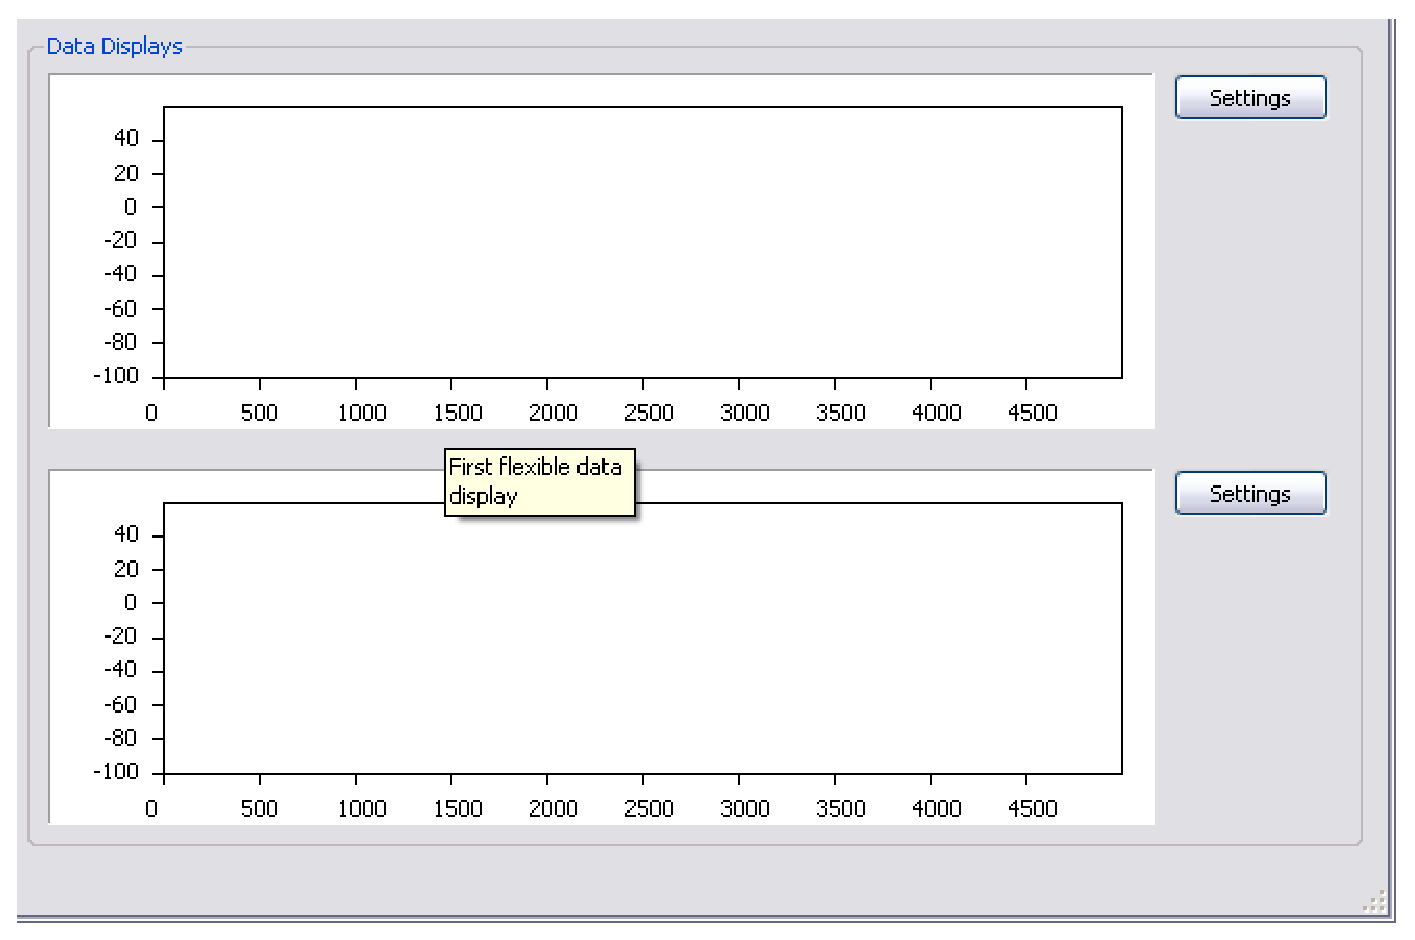
\includegraphics[scale=0.6]{graphBlock}
} \\[0.2cm]
The graph panels are controlled by the dialog that appears when
pressing ``Settings''. \\

\noindent
\parbox{0.62\textwidth}{
  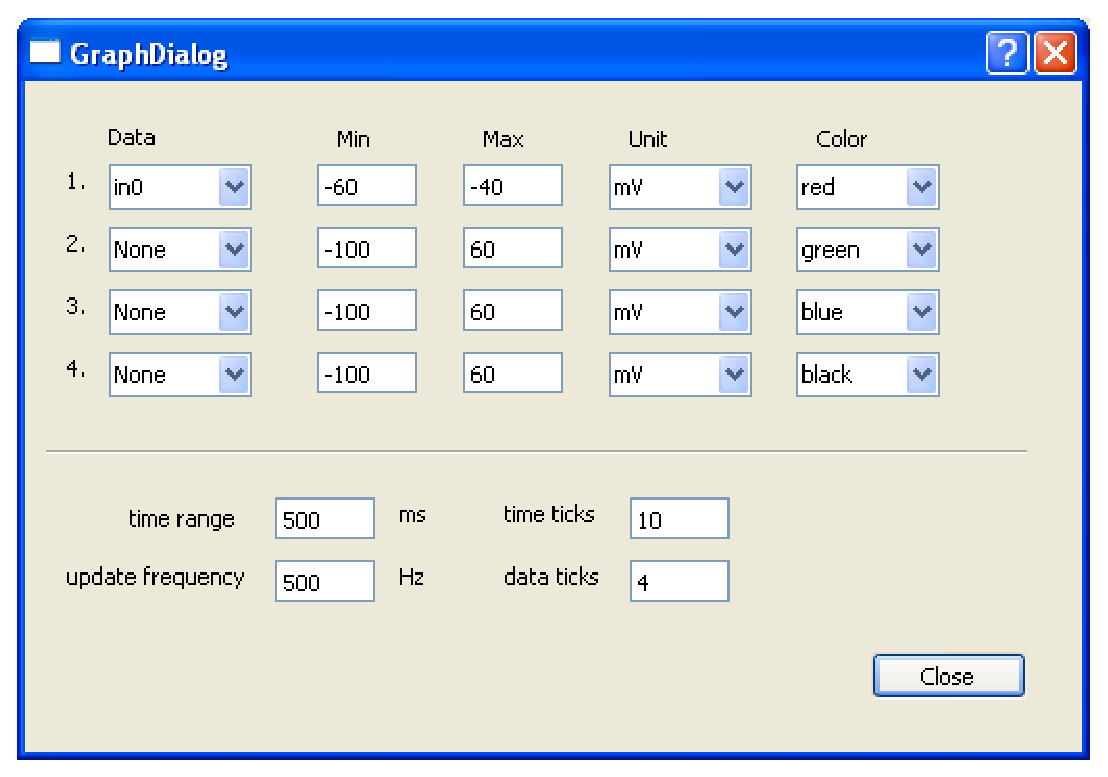
\includegraphics[scale=0.5]{graphDialog}
}
\hfill
\parbox{0.36\textwidth}{
The control elements are:
\begin{myitem}
\item Data column: Combo boxes to choose which data to display
\item Min: Minimum on the y axis for this data
\item Max: Maximum ion the y axis for this data
\item Unit: Units in which Min and Max are expressed
\item Color: Choice of color of the data trace.
\end{myitem}
}
\begin{myitem}
\item time range: The length of the x axis in ms
\item time ticks: Tumber of ticks on the x axis. 
\item update frequency: The rate with which points on the display are
  updated. Note that a too high rate will likely lead to an overload
  and subsequent freeze of the program. A more efficient and safe
  implementation of the displays is on the todo list.
\end{myitem}

\section{Experiment automation}

So far we have described how to cotrol StdpC 2007 using the graphical
user interface. Instead, or in addition, most parameters can be
controlled through a scripting mechanism. Through the
File$rightarrow$Load Script one can specify a script file. The script
file should contain three columns:
\begin{myenum}
\item A time in seconds when a certain event shall occur
\item A parameter name in clear text which shall be changed
\item A new value for the parameter in question
\end{myenum}
The value column can contain double precision numbers or integers
depending on the parameter being changed.

The script file will be read into a list of events in memory such that
changes to the file have no effect after the script was loaded.

The parameter names are the same as used when the state of the gui is
saved (``save protocol''). However, not all parameters can reasonably
changed while the clamp is running. A list of the most common
parameters on may want to change through scripting are given in the table. \\
\begin{table}
\begin{tabular}[t]{|ll|}
\hline
{\bf Name} & {\bf value range} \\
\hline
CSynp[i].ST.AMinus & double \\
CSynp[i].ST.tauMinus & double \\
CSynp[i].ST.APlus & double \\
CSynp[i].ST.tauPlus & double \\
CSynp[i].ST.Exponent & int \\
CSynp[i].ST.Shift & double \\
CSynp[i].ST.History & int \\
CSynp[i].ST.tableDt & double \\
CSynp[i].ST.tableDgMin & double \\
CSynp[i].ST.gMax & double \\
CSynp[i].ST.gMid & double \\
CSynp[i].ST.gSlope & double \\
CSynp[i].ODE.InitialP & double \\
CSynp[i].ODE.InitialD & double \\
CSynp[i].ODE.betaP & double \\
CSynp[i].ODE.betaD & double \\
CSynp[i].ODE.gamma & double \\ 
CSynp[i].ODE.eta & int \\
CSynp[i].ODE.highP & double \\
CSynp[i].ODE.lowP & double \\
CSynp[i].ODE.highD & double \\
CSynp[i].ODE.lowD & double \\
CSynp[i].ODE.gMax & double \\
CSynp[i].ODE.gMid & double \\
CSynp[i].ODE.gSlope & double \\
CSynp[i].gSyn & double \\
CSynp[i].VSyn & double \\
CSynp[i].tauSyn & double \\
CSynp[i].VThresh & double \\
CSynp[i].VSlope & double \\
CSynp[i].STD & 0-1 \\
CSynp[i].STDAmpl & double \\
CSynp[i].STDVThresh & double \\
CSynp[i].STDVSlope & double \\
CSynp[i].STDtauAmpl & double \\
CSynp[i].STDtau0 & double \\
CSynp[i].STDtauVThresh & double \\
CSynp[i].STDtauVSlope & double \\
CSynp[i].fixVpost & 0-1 \\
CSynp[i].Vpost & double \\
CSynp[i].Plasticity & 0-2 \\
ESynp[i].type & 0-1 \\
ESynp[i].gSyn & double \\
mhHHp[i].gMax & double \\
mhHHp[i].Vrev & double \\
mhHHp[i].mExpo & int \\
mhHHp[i].hExpo & int \\
mhHHp[i].Vm & double \\
mhHHp[i].sm & double \\ \hline
\end{tabular}
\quad 
\begin{tabular}[t]{|ll|}
\hline
{\bf Name} & {\bf value range} \\
\hline
mhHHp[i].Cm & double \\
mhHHp[i].taum & double \\
mhHHp[i].taumAmpl & double \\
mhHHp[i].Vtaum & double \\
mhHHp[i].staum & double \\
mhHHp[i].Vh & double \\
mhHHp[i].sh & double \\
mhHHp[i].Ch & double \\
mhHHp[i].tauh & double \\
mhHHp[i].tauhAmpl & double \\
mhHHp[i].Vtauh & double \\
mhHHp[i].stauh & double \\
abHHp[i].gMax & double \\
abHHp[i].Vrev & double \\
abHHp[i].mExpo & int \\
abHHp[i].hExpo & int \\
abHHp[i].maFunc & 0-2 \\
abHHp[i].mka & double \\
abHHp[i].mVa & double \\
abHHp[i].msa & double \\
abHHp[i].mbFunc & double \\
abHHp[i].mkb & double \\
abHHp[i].mVb & double \\
abHHp[i].msb & double \\
abHHp[i].haFunc & 0-2 \\
abHHp[i].hka & double \\
abHHp[i].hVa & double \\
abHHp[i].hsa & double \\
abHHp[i].hbFunc & 0-2 \\
abHHp[i].hkb & double \\
abHHp[i].hVb & double \\
abHHp[i].hsb & double \\
SGp.VSpike & double \\
SGp.spkTimeScaling & double \\
SGp.VRest & double \\
SGp.bdThresh & double \\
SGp.bdNUnder & double \\
SGp.bdNOver & double \\
SGp.period & double \\ 
SGp.SpikeNo & int \\
SGp.SpikeT[0] & double \\
SGp.SpikeT[1] & double \\
SGp.SpikeT[2] & double \\
SGp.SpikeT[3] & double \\
SGp.SpikeT[4] & double \\
SGp.SpikeT[5] & double \\
SGp.SpikeT[6] & double \\
SGp.SpikeT[7] & double \\
SGp.SpikeT[8] & double \\
SGp.SpikeT[9] & double \\ \hline
\end{tabular}
\end{table}

Please note that internally, all parameters and variables are in SI
units V, A, s, S, etc. The same applies to values in the script files. The variable $i$ in the variable names in the table has to be replaced by the appropriate number of the synapse or conductance, $i \in \{0, \ldots, 5\}$.

\section{User feedback} 
Please do give feedback if you found the software useful, buggy, or
have general comments or questions. Please send correspondence through
the sourceforge email or directly to T.Nowotny@sussex.ac.uk.
If you are interested in contributing to the future development please
do not hesitate to contact me as well.  
 
\section{Acknowledgments} 
 
The StdpC software would not exist without the early dynamic clamp
versions developed by Reynaldo D. Pinto and I (TN) am grateful to him for supplying the source code for further
development back then. I am also grateful to Attila Sz\"ucs for his excellent
suggestions for improving and extending the software and his tireless
testing of new and buggy versions.

\bibliographystyle{apalike}
\bibliography{master}
\end{document}
